% Options for packages loaded elsewhere
\PassOptionsToPackage{unicode}{hyperref}
\PassOptionsToPackage{hyphens}{url}
%
\documentclass[
  ignorenonframetext,
  aspectratio=169,
]{beamer}
\usepackage{pgfpages}
\setbeamertemplate{caption}[numbered]
\setbeamertemplate{caption label separator}{: }
\setbeamercolor{caption name}{fg=normal text.fg}
\beamertemplatenavigationsymbolsempty
% Prevent slide breaks in the middle of a paragraph
\widowpenalties 1 10000
\raggedbottom
\setbeamertemplate{part page}{
  \centering
  \begin{beamercolorbox}[sep=16pt,center]{part title}
    \usebeamerfont{part title}\insertpart\par
  \end{beamercolorbox}
}
\setbeamertemplate{section page}{
  \centering
  \begin{beamercolorbox}[sep=12pt,center]{part title}
    \usebeamerfont{section title}\insertsection\par
  \end{beamercolorbox}
}
\setbeamertemplate{subsection page}{
  \centering
  \begin{beamercolorbox}[sep=8pt,center]{part title}
    \usebeamerfont{subsection title}\insertsubsection\par
  \end{beamercolorbox}
}
\AtBeginPart{
  \frame{\partpage}
}
\AtBeginSection{
  \ifbibliography
  \else
    \frame{\sectionpage}
  \fi
}
\AtBeginSubsection{
  \frame{\subsectionpage}
}
\usepackage{amsmath,amssymb}
\usepackage{lmodern}
\usepackage{iftex}
\ifPDFTeX
  \usepackage[T1]{fontenc}
  \usepackage[utf8]{inputenc}
  \usepackage{textcomp} % provide euro and other symbols
\else % if luatex or xetex
  \usepackage{unicode-math}
  \defaultfontfeatures{Scale=MatchLowercase}
  \defaultfontfeatures[\rmfamily]{Ligatures=TeX,Scale=1}
\fi
\usetheme[]{metropolis}
% Use upquote if available, for straight quotes in verbatim environments
\IfFileExists{upquote.sty}{\usepackage{upquote}}{}
\IfFileExists{microtype.sty}{% use microtype if available
  \usepackage[]{microtype}
  \UseMicrotypeSet[protrusion]{basicmath} % disable protrusion for tt fonts
}{}
\makeatletter
\@ifundefined{KOMAClassName}{% if non-KOMA class
  \IfFileExists{parskip.sty}{%
    \usepackage{parskip}
  }{% else
    \setlength{\parindent}{0pt}
    \setlength{\parskip}{6pt plus 2pt minus 1pt}}
}{% if KOMA class
  \KOMAoptions{parskip=half}}
\makeatother
\usepackage{xcolor}
\newif\ifbibliography
\usepackage{graphicx}
\makeatletter
\def\maxwidth{\ifdim\Gin@nat@width>\linewidth\linewidth\else\Gin@nat@width\fi}
\def\maxheight{\ifdim\Gin@nat@height>\textheight\textheight\else\Gin@nat@height\fi}
\makeatother
% Scale images if necessary, so that they will not overflow the page
% margins by default, and it is still possible to overwrite the defaults
% using explicit options in \includegraphics[width, height, ...]{}
\setkeys{Gin}{width=\maxwidth,height=\maxheight,keepaspectratio}
% Set default figure placement to htbp
\makeatletter
\def\fps@figure{htbp}
\makeatother
\setlength{\emergencystretch}{3em} % prevent overfull lines
\providecommand{\tightlist}{%
  \setlength{\itemsep}{0pt}\setlength{\parskip}{0pt}}
\setcounter{secnumdepth}{5}
\ifLuaTeX
\usepackage[english]{babel}
\else
\usepackage[bidi=default]{babel}
\fi
\babelprovide[main,import]{russian}
\babelprovide[import]{english}
% get rid of language-specific shorthands (see #6817):
\let\LanguageShortHands\languageshorthands
\def\languageshorthands#1{}
\metroset{progressbar=frametitle,sectionpage=progressbar,numbering=fraction}
\makeatletter
\beamer@ignorenonframefalse
\makeatother
\ifLuaTeX
  \usepackage{selnolig}  % disable illegal ligatures
\fi
\IfFileExists{bookmark.sty}{\usepackage{bookmark}}{\usepackage{hyperref}}
\IfFileExists{xurl.sty}{\usepackage{xurl}}{} % add URL line breaks if available
\urlstyle{same} % disable monospaced font for URLs
\hypersetup{
  pdftitle={Научная презентация},
  pdfauthor={Рыжкова У. В.},
  pdflang={ru-RU},
  hidelinks,
  pdfcreator={LaTeX via pandoc}}

\title{Научная презентация}
\subtitle{Лабораторная №3}
\author{Рыжкова У. В.}
\date{25 февраля 2023}
\institute{Российский университет дружбы народов, Москва, Россия}

\begin{document}
\frame{\titlepage}

\hypertarget{ux438ux43dux444ux43eux440ux43cux430ux446ux438ux44f}{%
\section{Информация}\label{ux438ux43dux444ux43eux440ux43cux430ux446ux438ux44f}}

\begin{frame}{Докладчик}
\protect\hypertarget{ux434ux43eux43aux43bux430ux434ux447ux438ux43a}{}
:::::::::::::: \{.columns align=center\} ::: \{.column width=``70\%''\}

\begin{itemize}
\tightlist
\item
  Рыжкова Ульяна Валерьевна
\item
  студент 1-ого курса
\item
  профессор кафедры прикладной информатики и теории вероятностей
\item
  Российский университет дружбы народов
\item
  \href{mailto:1132226462@pfur.ru}{\nolinkurl{1132226462@pfur.ru}}
\item
  \url{https://bl1nulya.github.io/ru/}
\end{itemize}
\end{frame}

\hypertarget{ux432ux44bux43fux43eux43bux43dux435ux43dux438ux435-ux43bux430ux431ux43eux440ux430ux442ux43eux440ux43dux43eux439-ux440ux430ux431ux43eux442ux44b}{%
\section{Выполнение лабораторной
работы}\label{ux432ux44bux43fux43eux43bux43dux435ux43dux438ux435-ux43bux430ux431ux43eux440ux430ux442ux43eux440ux43dux43eux439-ux440ux430ux431ux43eux442ux44b}}

\begin{frame}{Выполнение лабораторной работы}
\begin{enumerate}
\item
  Заданием является составить отчёт предыдущей лабораторной работы. Увы,
  я делала её с опозданием и совершенно забыла о скриншотах (надеюсь,
  скринкаст с комментариями решит этот недочёт)
\item
  Поскольку я уже являюсь пользователем github и в прошлом семестре
  настроила систему git, перехожу к шагу создания pgp ключа.
\end{enumerate}

\begin{figure}
\hypertarget{fig:001}{%
\centering
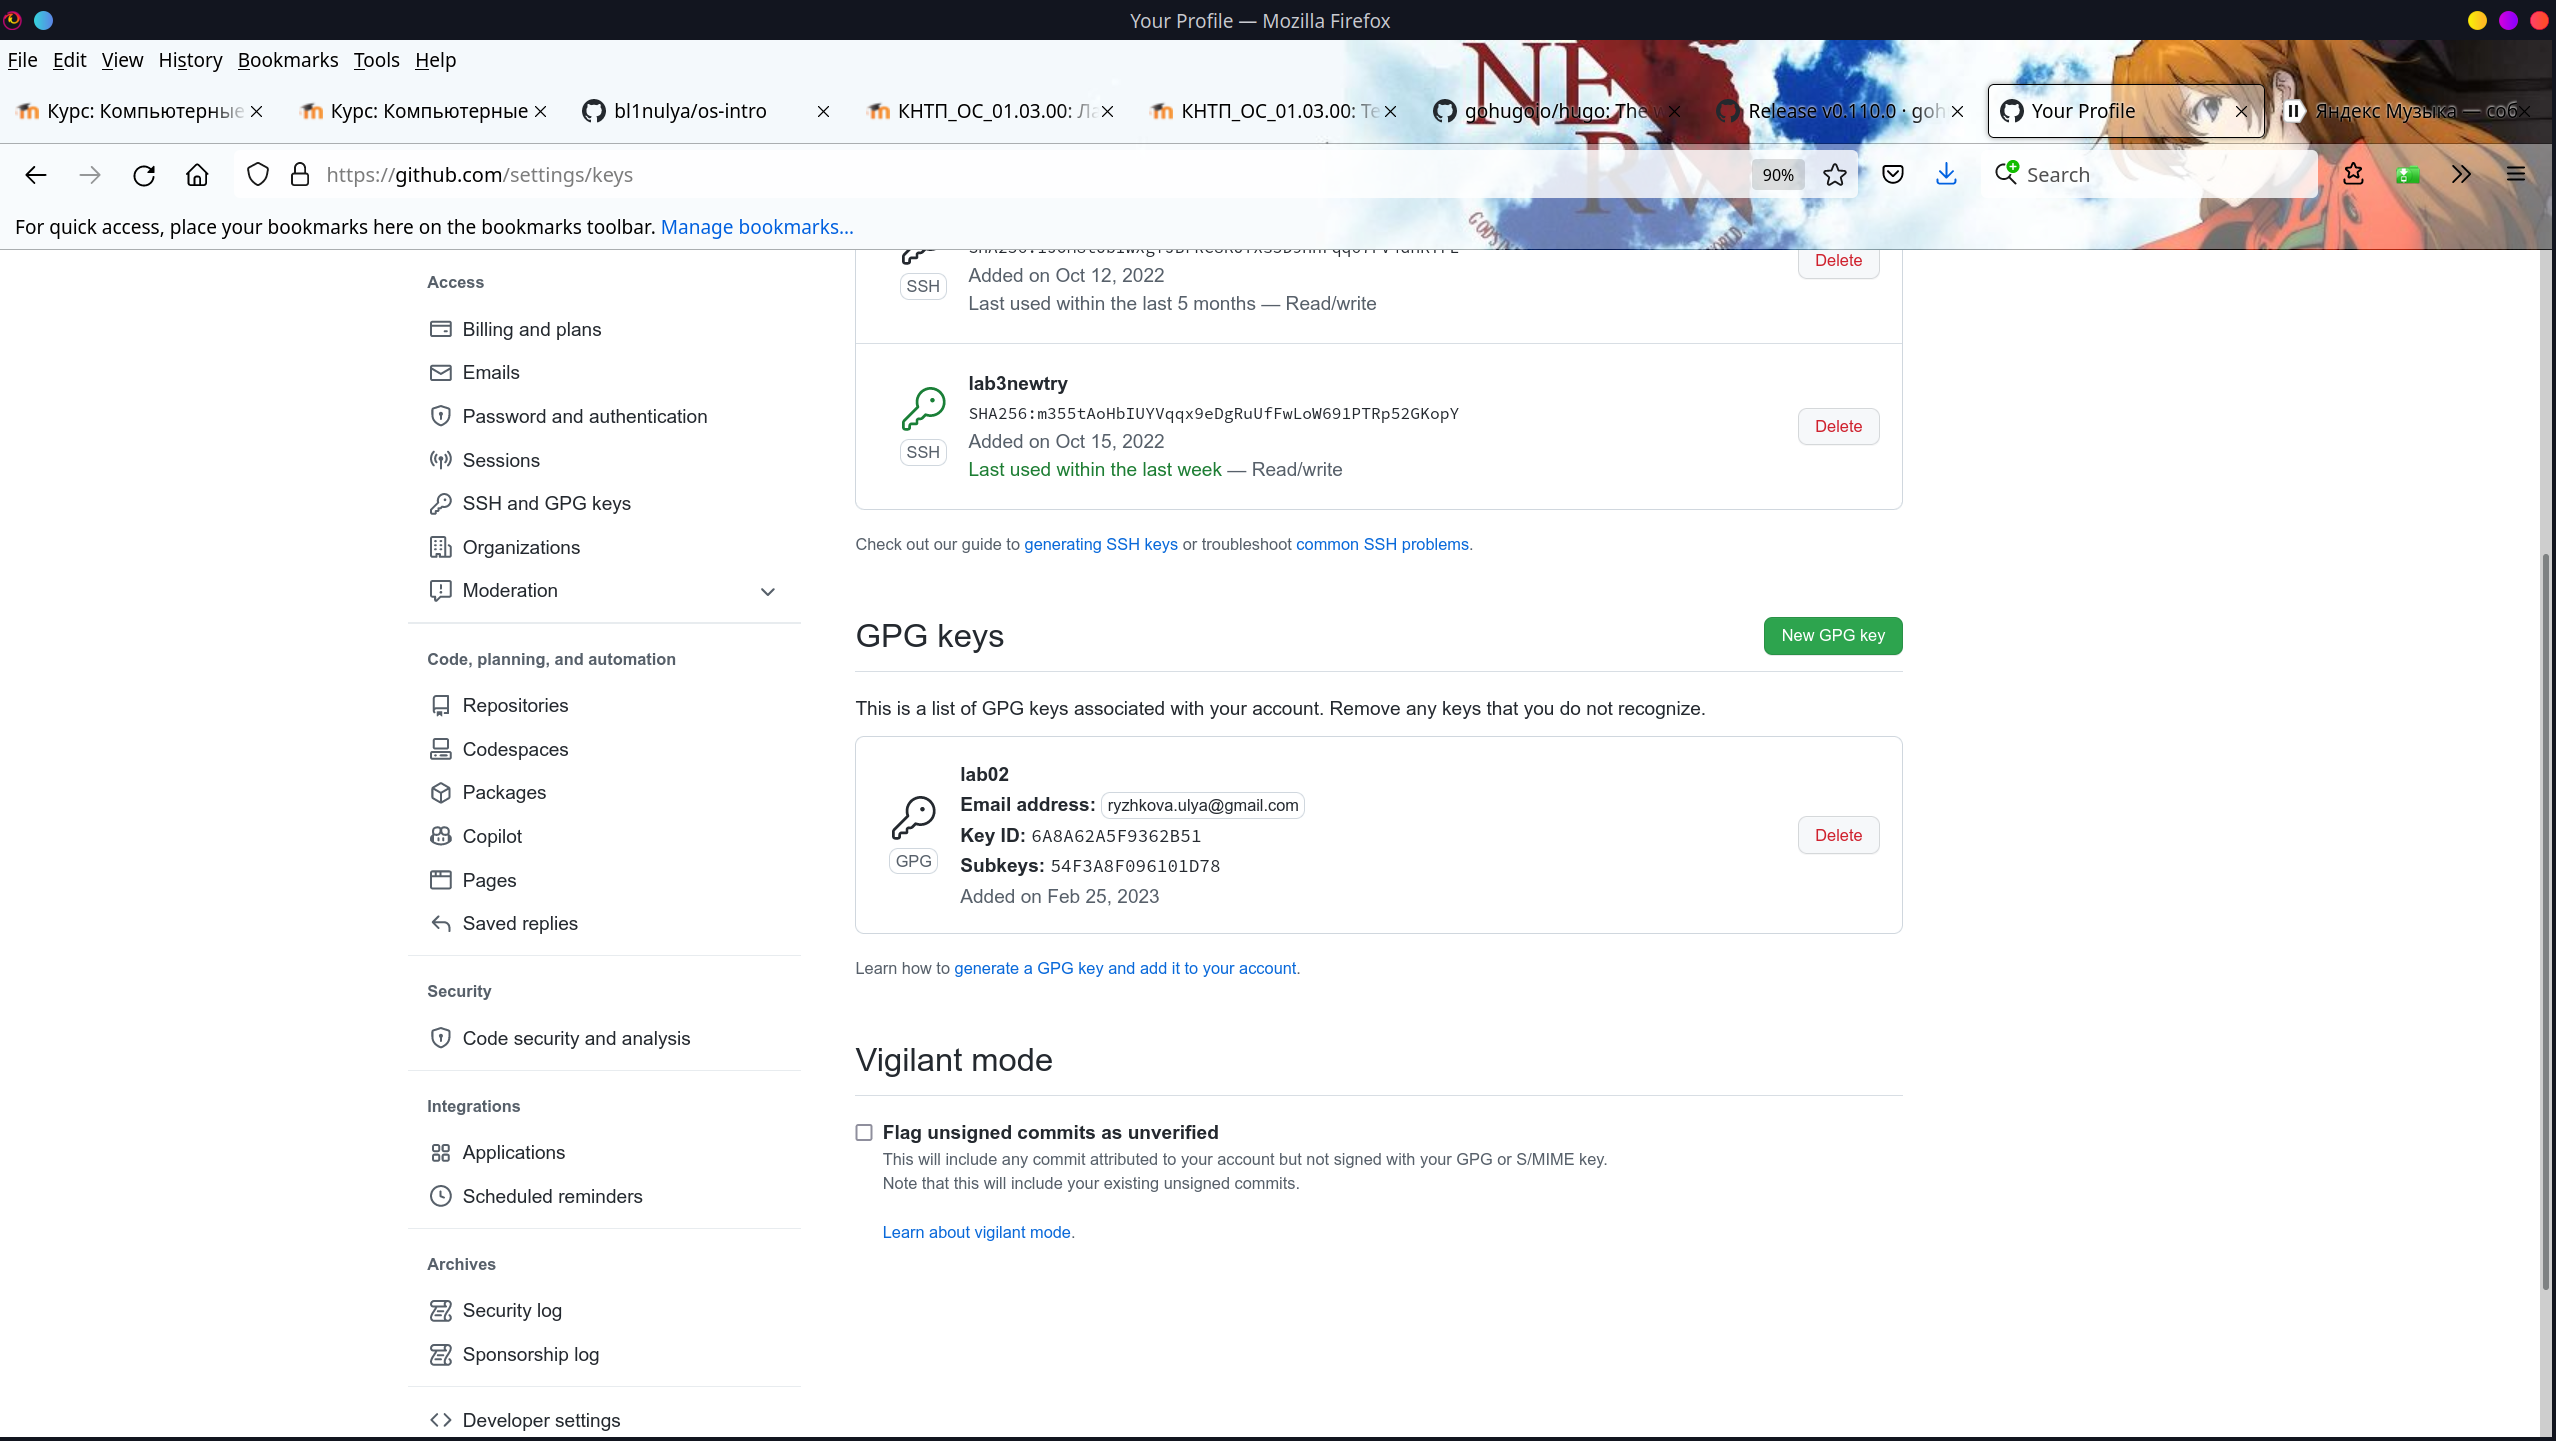
\includegraphics[width=1\textwidth,height=\textheight]{image/1.png}
\caption{Подключенный pgp ключ}\label{fig:001}
}
\end{figure}

\begin{enumerate}
\setcounter{enumi}{2}
\item
  Настроила подпись коммитов.
\item
  С помощью шаблона создаю репозиторий для проходимого в этом семестре
  курса.
\end{enumerate}

\begin{figure}
\hypertarget{fig:002}{%
\centering
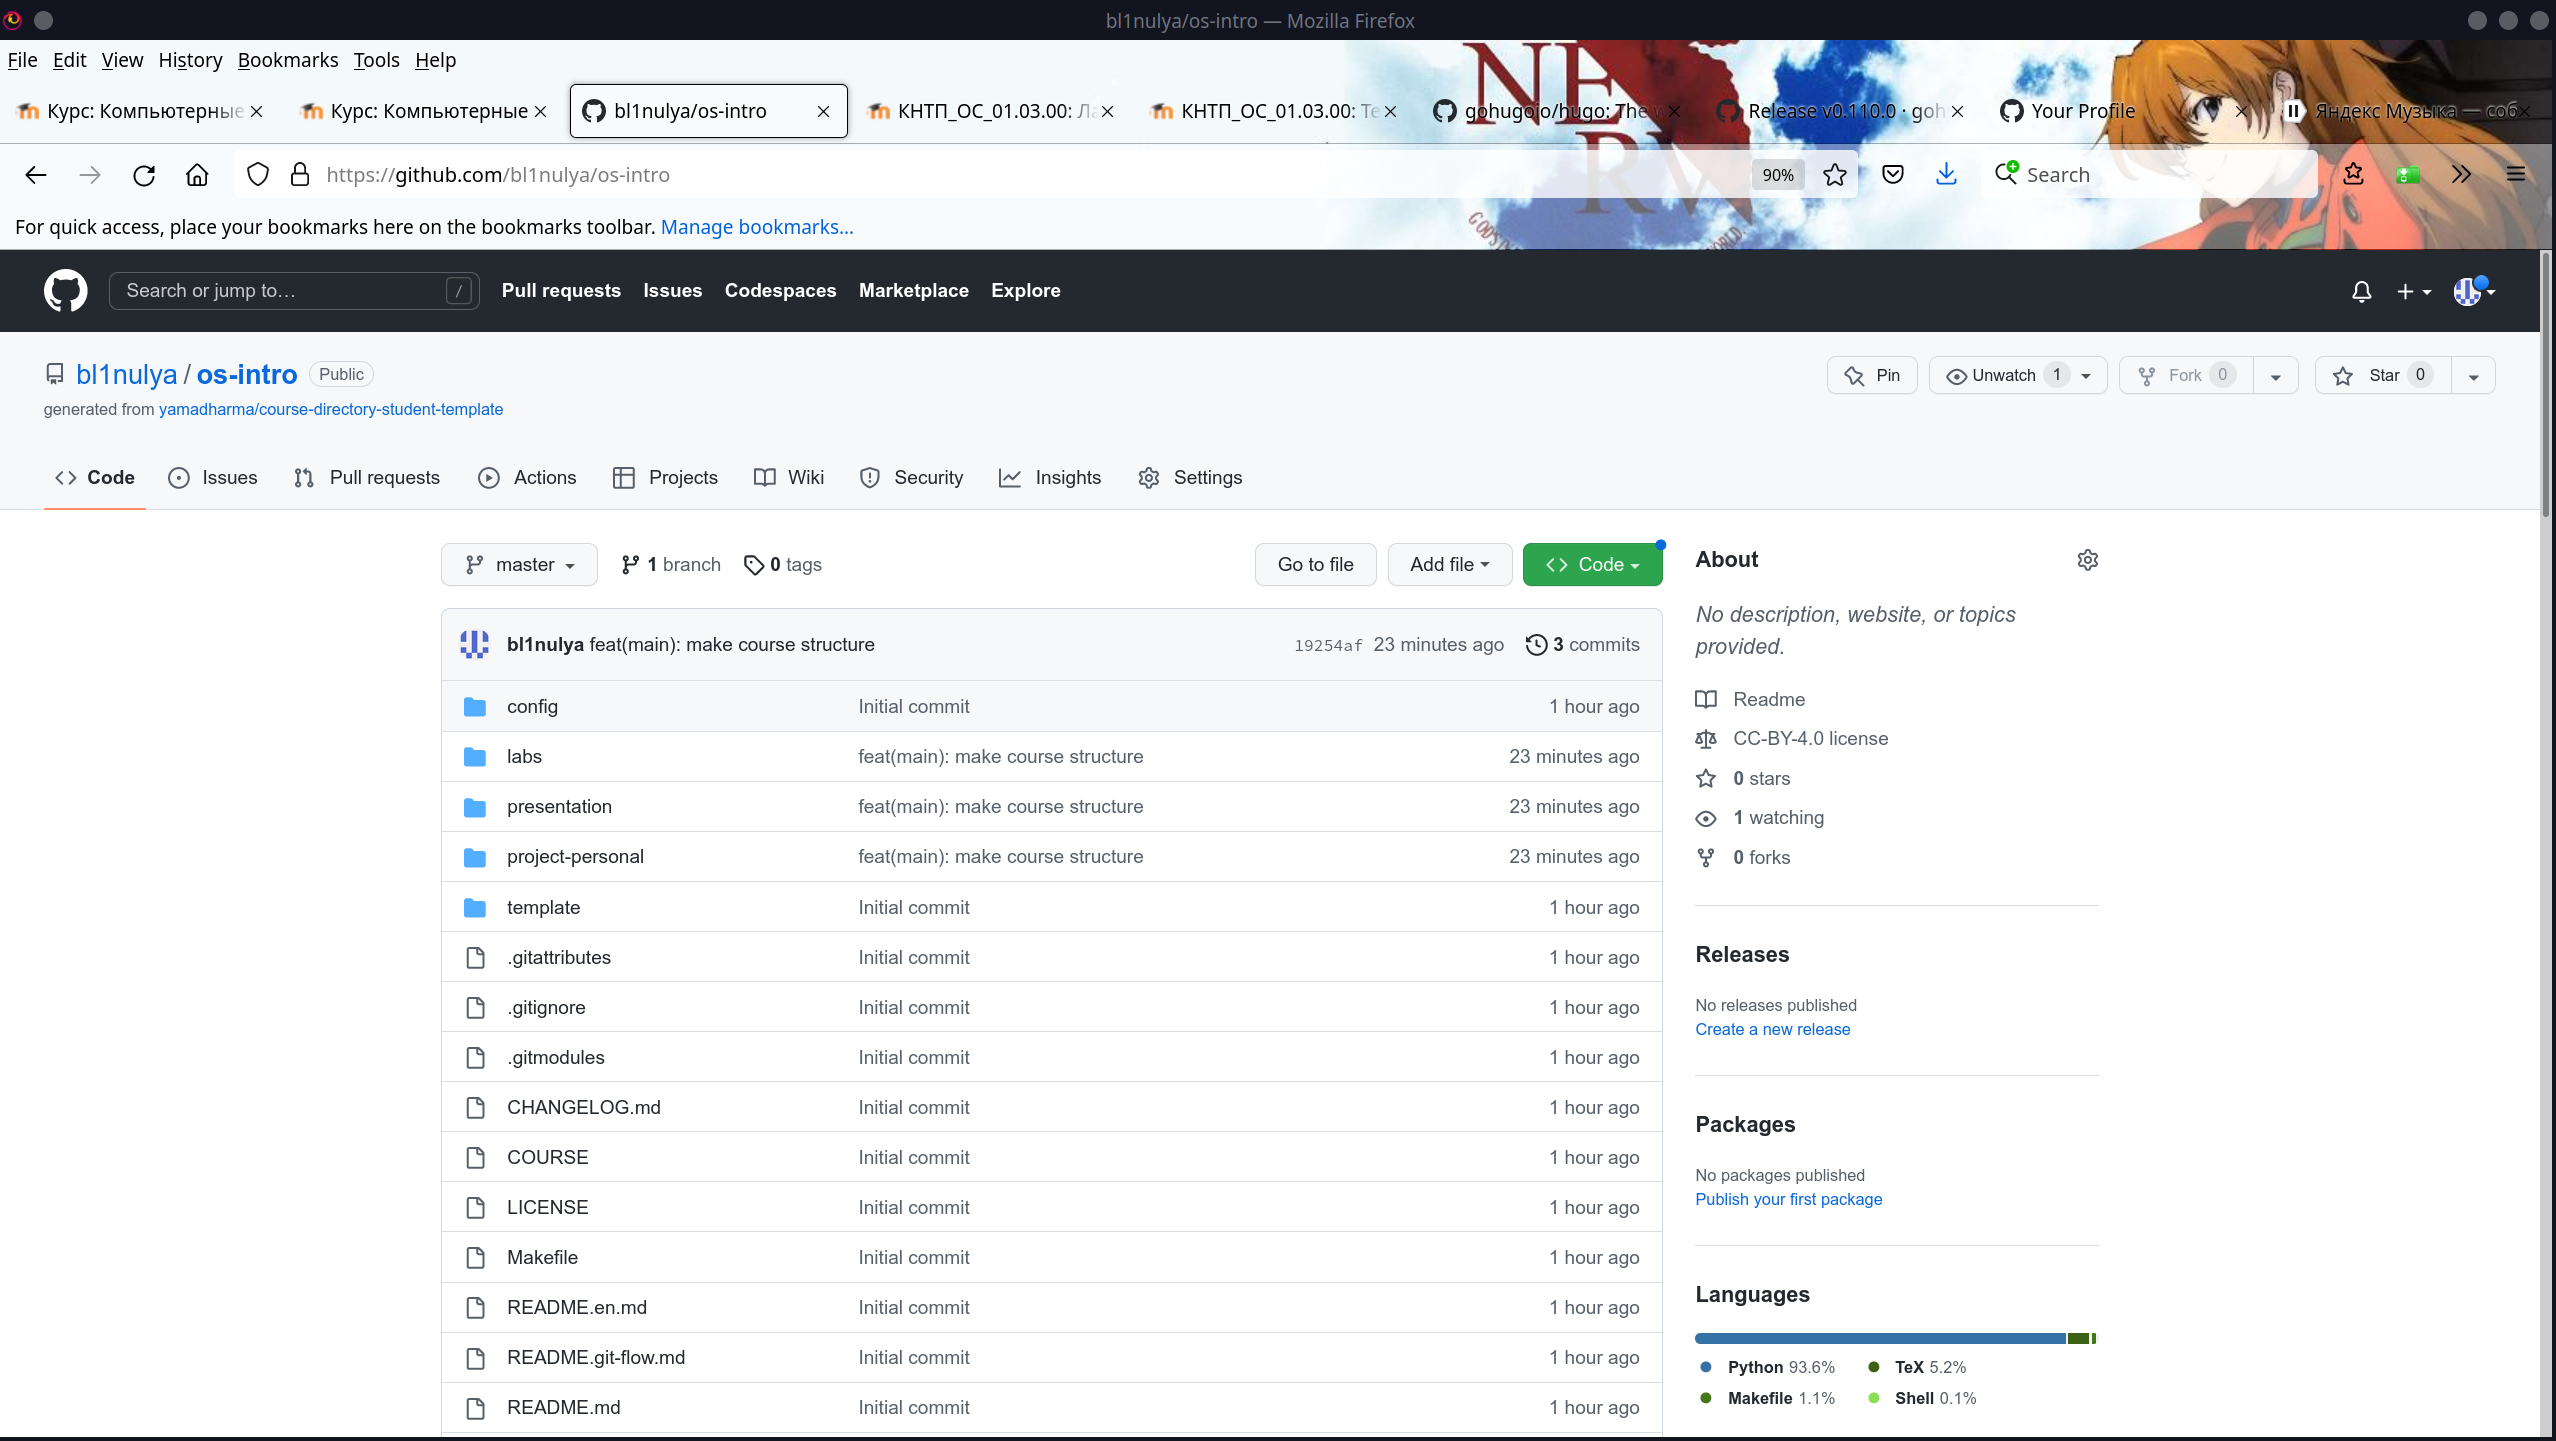
\includegraphics[width=1\textwidth,height=\textheight]{image/2.png}
\caption{Новый репозиторий}\label{fig:002}
}
\end{figure}

\begin{enumerate}
\setcounter{enumi}{4}
\tightlist
\item
  Удаляю лишние файлы и создаю необходимые каталоги с помощью команды
  make. Отправляю файлы на сервер.
\end{enumerate}

\begin{figure}
\hypertarget{fig:003}{%
\centering
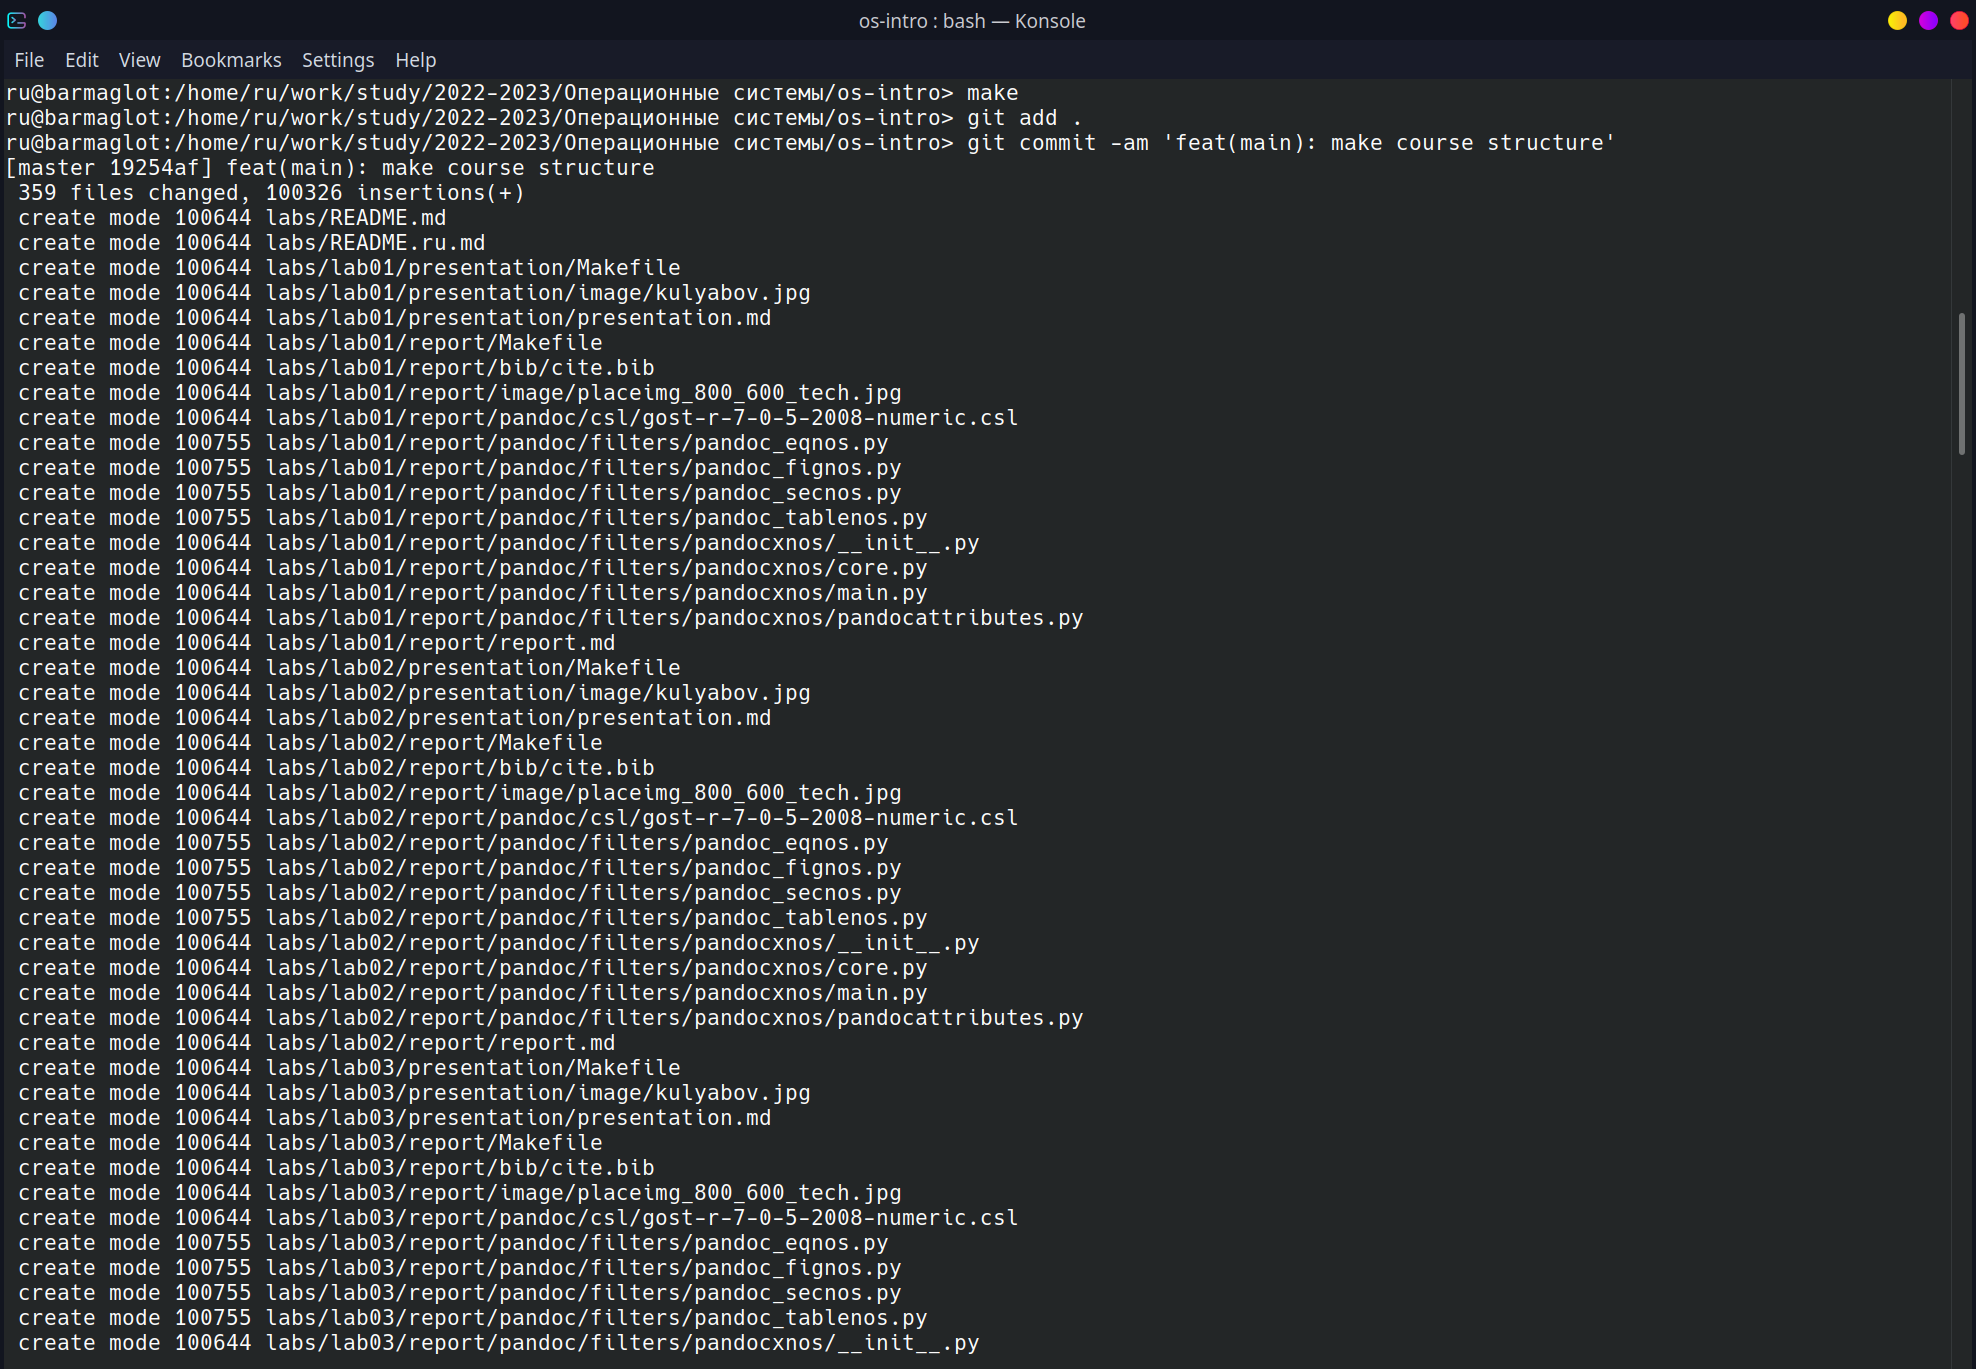
\includegraphics[width=1\textwidth,height=\textheight]{image/3.png}
\caption{Создание каталогов и загрузка файлов на сервер}\label{fig:003}
}
\end{figure}
\end{frame}

\hypertarget{ux432ux44bux432ux43eux434ux44b}{%
\section{Выводы}\label{ux432ux44bux432ux43eux434ux44b}}

\begin{frame}{Выводы}
Я ознакомилась с языком разметки Markdown.
\end{frame}

\end{document}
